\documentclass[a4paper,11pt]{article}

%% PREAMBLE %%

% Packages
\usepackage[utf8]{inputenc} % UTF-8 is a good thing I guess
\setcounter{secnumdepth}{0}
\usepackage[a4paper, total={150mm, 225mm}]{geometry} % use reasonable amount of the page
\usepackage{amsmath}  % allows unnumbered equations
\usepackage{textcomp} % explicitly imported to calm gensymb
\usepackage{gensymb}  % gives degree sign
\usepackage{tikz}     % allows drawing pretty diagrams
\usepackage{pgfplots} % allows graphs and plots
\usepackage{graphicx} % allows images
\usepackage{pdfpages} % allows to import other PDF pages
\usepackage{float}

%Prettifying packages
\usepackage[document]{ragged2e}
\usepackage[margin=1cm]{caption} % spacing for captions, 1cm in from border
\usepackage{subcaption} 
\usepackage{fancyhdr}
\pagestyle{fancy}
\usepackage[normalem]{ulem}
\usepackage{colortbl}
\usepackage{xcolor}
\usepackage{listings}

%make numbers not selectable
\usepackage{accsupp}
\renewcommand{\thelstnumber}{% Line number printing mechanism
  \protect\BeginAccSupp{ActualText={}}\arabic{lstnumber}\protect\EndAccSupp{}
}
\usepackage[T1]{fontenc}
\usepackage[framed,numbered]{matlab-prettifier} %print pretty code
\usepackage{epstopdf}


% Titlepage variables
%\title{SA1: Interim Report 1}
%\author{Paul Wernicke (pw444)\\Jonathan Collins (jc2071)}
%\date{May 2020}

\lhead{Final Report}
\rhead{Jonathan Collins}
\lfoot{jc2071}

%% DOCUMENT %%
\pagenumbering{gobble}
\begin{document}
%\maketitle
\begin{titlepage}
    \begin{center}
 
        \LARGE
        SA1: Aircraft Wing Analysis
        
        \vspace{0.1cm}
        
        \LARGE
        
        Interim Report 1
        
        \vspace{0.4cm}
        
        \large
        
        Jonathan Collins \& Paul Wernicke
        
        \vspace{0cm}
        
        Homerton College
        
        \vspace{0.3cm}
        
        Easter Term 2020
        
        \vspace{0.5cm}
        
        %\large
        
        %\textbf{Abstract}
        
        %\justify
        
        %\normalsize
        %I don't think we really need an abstract.
        %\tableofcontents
        \lstlistoflistings
    \end{center}
\end{titlepage}
\pagenumbering{arabic}

\section{Plan}
\justify

1) title page
2) abstract - Final airfoil data (max L/D, operating alpha...), ro references, important $findings$ and what we did. short
3) Introduction -  why we are doing it, what else has been done
4) Validity of numerical model
    4.a Initial comparison with experimental data - surface roughness, separation bubbles, lift inviscid, drag turbulent, no accounting for compressibility and fast speed is like mach > 0.05
    4.b refinements - the gamma fix, visual turbulent separation warning on wasg,but still only a 1st order bodge as not fully integrate BL and inviscid flow
    
5) Design Process

  5.a) Design philosophy - which curves we focus on to asses things, l/d vs α, cp vs x/c, cl vs cd (google), 

  5.b) Low speed story start with naca 15
    5.a.i. 5 revisions, what we are improving in each case, based on physical process( cp and is it separating)
    5.a.ii final characteristics (incl at high speed)

  5.c) High speed story naca 12
    5.b.i  5 revisions, what we are improving in each case, based on physical process( cp and is it separating)
    5.b.ii final characteristics (incl at low speed)
    
6) Extension maybe

7) Conclusion
    




Should address:
 - The validity and accuracy of the numerical model
 - the design process by which you reached your optimum aerofoil sections
 - the optimum sections and their aerodynamic characteristics
 - the physical processes which determine the aerodynamic characteristics of the optimum and non-optimum sections
 - the reliability of results

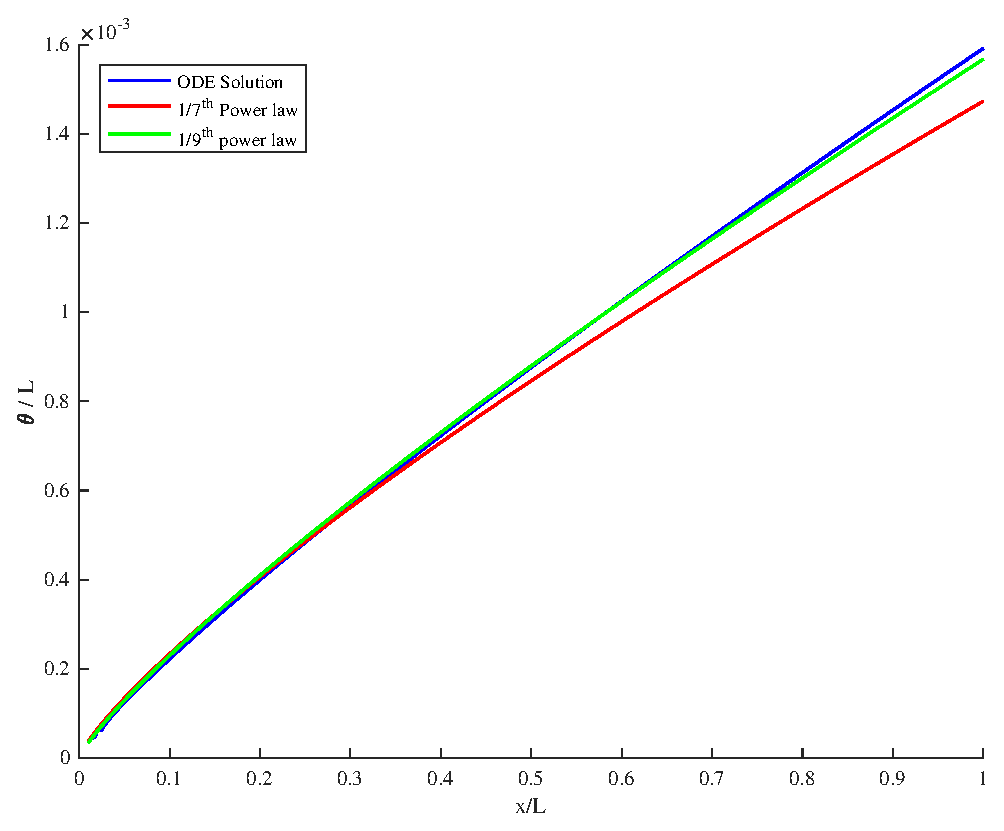
\includegraphics[scale=0.80]{graphs/e4g1.eps}

\end{document}